\documentclass[10pt]{article}\usepackage[margin=.65in]{geometry}\usepackage[T1]{fontenc}\usepackage{graphicx}\setlength{\parindent}{0pt}\setlength{\parskip}{7pt}\sloppy\begin{document}{\large Independent stored-input extraction review}\par Independent replay and source inspection recorded passed, faithful\_scoped and validated\_scoped for five main declarations and seven producer controls at commit 1ef3c786cc1ac3041bf584a80b15bf9869735f64. Five target modules were freshly compiled. Twelve producer and three reviewer named axiom readbacks passed; the false theorem exited 1 and three malformed checker inventories were rejected. This archive preserves the completed review without new proof execution.\par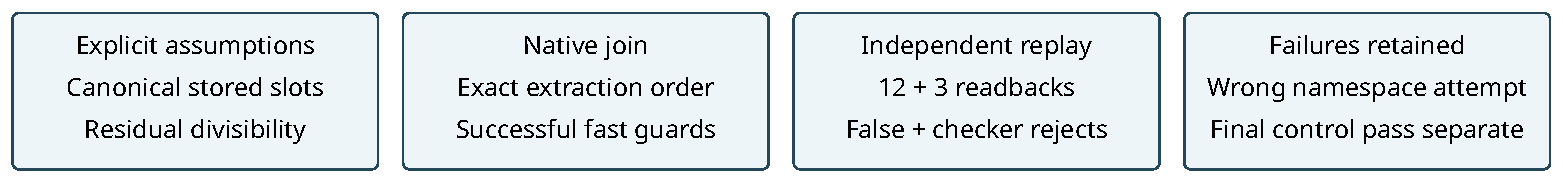
\includegraphics[width=\linewidth]{diagram.pdf}\par Source-conditioned construction. WellFormed assumes degree at most two, exact capacities three/two, canonicality in every slot, active leading one and decoded residual divisibility. Nonzero inactive padding is allowed; noncanonical padding is not. The accessor proof handles degrees zero, one and two and trims V. Extraction follows native qa,ra,sa,ta,qb,rb,sb,tb ordering; total getD defaults cannot be reached after capacity decomposition. Residual hypotheses follow by rewriting WellFormed. The decoded vpB equality is sufficient for the residual join, without requiring an unproved list identity.

Fast branch scope. stored\_fast\_calls is conditional on degree-two wellformed inputs, canonical degree-five f, prime 2$<$p$<$2\textasciicircum{}31 and the actual nonzero norm/s1 guards. Its modeled arithmetic corresponds to n=1 with no tables. Native validation admits odd p$>$=5 below2\textasciicircum{}31; the helper also admits p=3 without claiming native validation accepts it. The result gives successful modeled quotient/remainder equations and canonical normalized lists with support length three/leading one and ordinate length at most two. Full dispatch is a later joint.

Controls and retained failure. Reviewer controls check unique-word extraction order, rejection of active leading two, and rejection of inactive coefficient 17 modulo17. Producer F17 controls establish input residuals and nonzero guards; returned lists are existential, not a measured native trajectory. The first reviewer control used the wrong namespace ScaleTrim.Canon and exited 1 with an unresolved goal and sorryAx readback. That source/output remain in reviewer-attempt1 as rejected evidence. Correcting only the namespace to MonicRemainder.Canon produced the accepted final controls. Producer failures remain in the separate producer archive.

Provenance and cache boundary. The full native SHA256 is bound in status.json and the retained source inventory. Review inspected the exact published source and main fdb5f599e9d35584b1df9466d3c9a46f10d2e89e separately: native bytes matched. The original failed producer attempt bound live source; later successful attempts bound the immutable private snapshot with the same native hash. Direct helper/compiler inputs were checked before and after. Deeper retained union inventories were checked before and after replay; they were not a newly collected full dependency snapshot. Imported binaries were reused; no independent binary/kernel rechecker or exclusion of transient concurrent edits is claimed.

Independence and evidence. The non-author reviewer inherited task history, consulted no sibling verdict, and reused earlier scripts only as mechanics. review/REVIEW.md and review/review.json contain sources read and per-claim outcomes; sources, logs and exact bindings are archived. Native validator equivalence, physical execution, allocation/counters, whole dispatch and Picard classes remain outside this review. No scientific status, timing, cohort or budget changed. The editable diagram shows reviewed joins rather than performance data. Next is full source-ordered dispatch composition; canonical scientific graphs remain unchanged.
\end{document}